\section{Results}
\label{sec:results}

\subsection{Power Comparisons}
\label{sub:power_comparisons}

Figure~\ref{fig:simulatedGeneRealData} displays the mean empirical power for each test under various scenarios for the 50 randomly selected genes.
In each scenario I considered a single causal region of size $\gamma$.
The size of the causal region was defined relative to the total gene size (given in percentage).
For example, given a gene with 10 rare variants and $\gamma=0.2$ then the first $2$ mutations defined as causal mutations.
Empirical power was compared between Skat, SkatO, KS, CMC, Burden and KS-Burden under different assumed effect sizes ($r^2=(0.002, 0.006, 0.009)$).
The selected $50$ genes had at least $6$ genetic variants and maximal $60$ with a median of $8.5$ variants.

All tests were affected by the size of the causal cluster.
As expected, KS and Skat greatly lose statistical power when $\gamma$ increases.
The KS test showed greater statistical power between $\gamma=0.2$ and $\gamma=0.6$ than Skat, but lost significant power when $\gamma$ increases.
Further, KS performed only slightly better than Skat at $\gamma=0.2$.
Interestingly the simple KS test also outperformed SkatO at $\gamma=0.4$, but to a lesser extend.
Both burden tests, that is CMC and Burden, demonstrated an monotonic increase in statistical power over $\gamma$.
Thus suffering from a reduction in power at $\gamma=0.2$ but outperformed all other tests when all variants were disease causing.

Omnibus tests, that is SkatO and KS-Burden, are relatively unaffected by the change in $\gamma$ and KS-Burden is able to outperform SkatO across scenarios.
However, while the mean power of SkatO remains rather stable across all scenarios, KS-Burden has a slight reduction in power at $\gamma=0.2$.

Assessment of the correlation between test statistics of KS and Burden test across assessed genes under the null was with $r=0.03$ small.
Thus providing some evidence for the indecency of both tests. %TODO need to check this correlation again 

\begin{figure}[ht!]
  \centering
  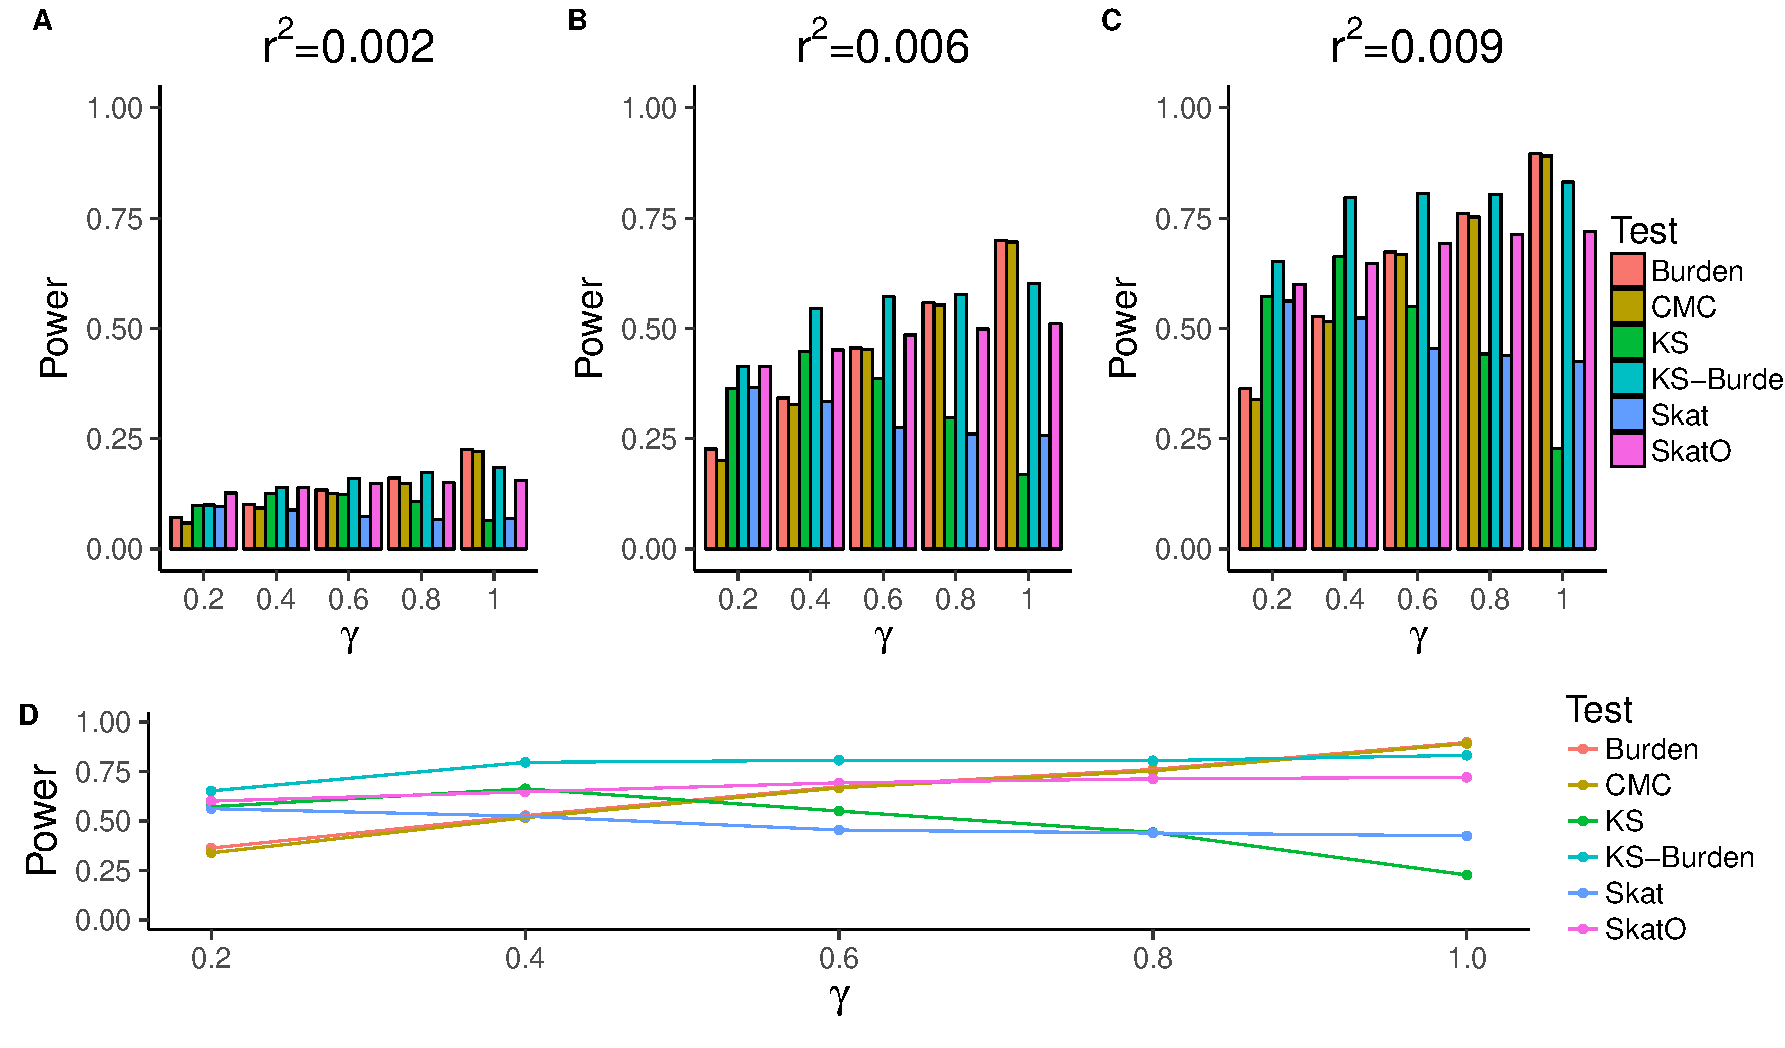
\includegraphics[width=0.8\linewidth]{ksburden/figures/combined_power_analysis.pdf}
  \caption{Estimated mean statistical power for five different causal cluster size $\gamma$ over selected 50 genes.
    (A-C) Different power estiamtions for each rare variant association test for $r^2=0.002, 0.006, 0.009$.
    The percentage of causal mutations $\gamma$ are on the corresponding x-axis, while empirical power is on the y-axis.
    (D) Relative change in empirical power over changes in $\gamma$ for each assessed test.\label{fig:simulatedGeneRealData}}
\end{figure}


\subsection{UKBioBank -- Aggression}
\label{sub:ukbiobank_aggression}

The QQ-plot for all tests is displayed in Figure~\ref{fig:qqplot_ksburden} and the top $10$ genes are shown in Table~\ref{tab:top_ksburden}.
